\documentclass[12pt]{article}

%%%%%%%%%%%%%%%%%%%%%%%%%%%%
%%%%%%%%%%%%%%%%%%%%%%%%%%%%
% Load in packages
\usepackage{amsmath}
\usepackage{amssymb}
\usepackage{hyperref}
\usepackage{graphicx}
\usepackage[top=1in, bottom=1in, left=1in, right=1in]{geometry}

%%%%%%%%%%%%%%%%%%%%%%%%%%%%
%%%%%%%%%%%%%%%%%%%%%%%%%%%%

\begin{document}

\begin{center}
\Large Chapter 7 Practice Problems Solutions

\medskip

\normalsize Elements of Microeconomics

\medskip

\small Discussion section 4
\end{center}

\medskip

\section*{Question 1}
Consider Figure 1 from chapter 7 in the textbook.

\vspace{2mm}

What happens to the auction price if there is only one record at auction but there is another buyer, Yoko, who also values the record at \$100?

\vspace{2mm}

\textbf{Answer:}

\vspace{2mm}

Now the auction price will be bid up to \$100.

\vspace{2mm}

Before, once the auctioneer reached \$80, all three other bidders dropped out and John could buy the record. It is too expensive for any of the other purchasers, but the buyer cannot get a higher price from John.

\vspace{2mm}

Now, when the auctioneer calls out \$80, Yoko is willing to pay \$81, since the price is still below her willingness to pay of \$100. But then John calls out \$82, for the same reason; this process repeats until they reach a price of \$100.

\section*{Question 2}
Consider the market for coffee in figure \ref{fig:coffee1}.

\begin{figure}
    \centering
    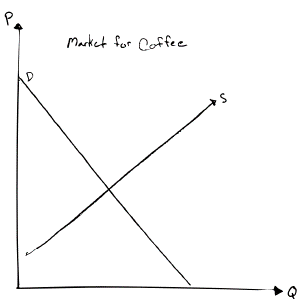
\includegraphics[width=.5\textwidth]{../../figs/coffee1.png}
    \caption{Coffee market}
    \label{fig:coffee1}
\end{figure}

\subsection*{Part A}
Draw the total surplus at the market equilibrium, identifying consumer surplus and producer surplus.

\vspace{2mm}

\textbf{Answer:}

\vspace{2mm}

Your graph should look like figure \ref{fig:coffee2}. Consumer surplus is given by $A_1$, showing the difference between the market price and the willingness to pay at each point. The producer surplus is given by $A_2$, showing the difference between the market price and producer cost at each point. The total surplus is just $A_1 + A_2$.

\vspace{2mm}

\begin{figure}
    \centering
    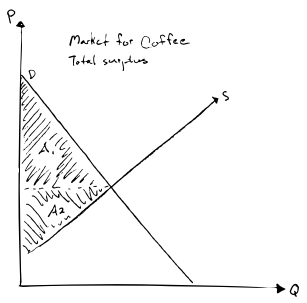
\includegraphics[width=.5\textwidth]{../../figs/coffee2.png}
    \caption{Coffee market}
    \label{fig:coffee2}
\end{figure}

\vspace{2mm}

\subsection*{Part B}
Now suppose the government imposes a tax on consumption of coffee.

\vspace{2mm}

\begin{enumerate}
    \item Illustrate the impact of the tax on the market equilibrium; what happens to P and Q?
    \item What happens to consumer surplus?
    \item Producer surplus?
    \item Total surplus?
\end{enumerate}

\vspace{2mm}

\textbf{Answer:}

\vspace{2mm}

The new market equilibrium is given in figure \ref{fig:coffee4}. The tax shifts the demand curve to the left; now consumers are paying $P_c$, but producers only receive $P_s$. The new equilibrium price and quantity are lower.

\begin{figure}
    \centering
    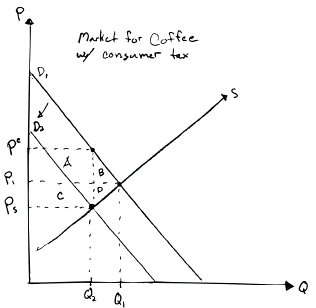
\includegraphics[width=.5\textwidth]{../../figs/coffee4.png}
    \caption{Coffee market with consumer tax}
    \label{fig:coffee4}
\end{figure}

The effects on surplus are:
    \begin{itemize}
        \item Consumer surplus decreases by $A + B$
        \item Producer surplus decreases by $C + D$
        \item Government revenue is given by $A + C$
        \item $(A+C) - (A+B) - (C+D) = -(B + D)$ is deadweight loss
    \end{itemize}

\vspace{2mm}

\subsection*{Part C}
Now suppose the government provides a subsidy to producers for each cup of coffee they sell, and answer the same questions as in Part B.

\vspace{2mm}

\textbf{Answer:}

\vspace{2mm}

The new market equilibrium is given in figure \ref{fig:coffee3}. The tax shifts the supply curve to the right; now consumers are paying $P_c$, but producers actually receive $P_s$. The new equilibrium price is lower and quantity is higher.

\begin{figure}
    \centering
    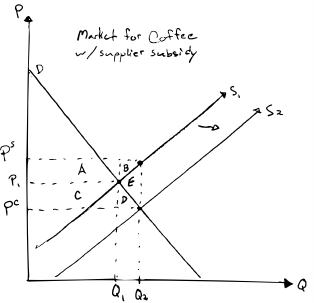
\includegraphics[width=.5\textwidth]{../../figs/coffee3.png}
    \caption{Coffee market with producer subsidy}
    \label{fig:coffee3}
\end{figure}

The effects on surplus are:
    \begin{itemize}
        \item Consumer surplus increases by $C + D$
        \item Producer surplus increases by $A + B$
        \item Government spends $ A + B + C + D + E $
        \item $(C+D) + (A + B) -  (A + B + C + D + E) = - E$ is deadweight loss
    \end{itemize}

\vspace{2mm}

\subsection*{Part D}
With the two policies, does the government increase or decrease total surplus? How does the change in total surplus compare to the change in government revenue?

\vspace{2mm}

\textbf{Answer:}

\vspace{2mm}

The tax decreases surplus for both consumers and producers. In the tax, the government revenue is strictly smaller than the decrease in surplus; the difference is the deadweight loss. 

\vspace{2mm}

The subsidy increases surplus for both consumers and producers. However, the revenue that the government must spend to acheive this increase is strictly larger; the difference is the deadweight loss from the policy.

\vspace{2mm}

The take-away is that in our simplistic model of a perfectly competitive market, there is always some deadweight loss.

\section*{Question 3}
Let's consider the market for iPhones.

\subsection*{Part A}

Is the demand for iPhones elastic or inelastic? What about supply?

\vspace{2mm}

\textbf{Answer:}

\vspace{2mm}

You could argue for either elastic or inelastic supply and demand. Demand may be elastic because there are close substitutes, such as android or Huawei phones, and  the fact that a smartphone is in some sense a luxury good. Demand may be inelastic because in reality, having a smartphone is necessary for communication and work in 21st century America, and many people are ``locked in'' to Apple's technology infrastructure. Supply may be elastic because Apple makes millions of these items and can scale-up or down supply, but may be inelastic because it is a capital-intensive production process with large investments in technological research.

\subsection*{Part B}

Assume supply and demand are both fairly elastic (slope around 1). Illustrate the impact of a decrease in the cost of production, and show the change to surplus.

\vspace{2mm}

\textbf{Answer:}

\vspace{2mm}

The original market is given by figure \ref{fig:iphone1}. A decrease in the cost of production shifts the supply curve down and to the left, and increases total surplus for both consumers and producers, shown in figure \ref{fig:iphone2}.

\begin{figure}
    \centering
    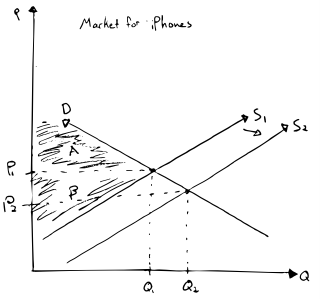
\includegraphics[width=.5\textwidth]{../../figs/iphone1.png}
    \caption{Market for iPhones}
    \label{fig:iphone1}
\end{figure}

\begin{figure}
    \centering
    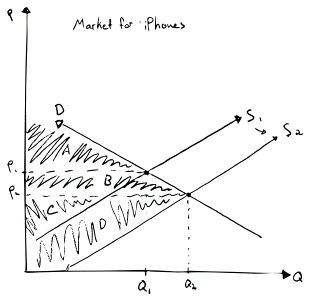
\includegraphics[width=.5\textwidth]{../../figs/iphone2.png}
    \caption{Change to surplus in the market for iPhones}
    \label{fig:iphone2}
\end{figure}

\subsection*{Part C}

Now suppose that the demand curve for iPhone is very inelastic (close to vertical), and answer the same questions.

\vspace{2mm}

\textbf{Answer:}

\vspace{2mm}

The original market is given by figure \ref{fig:iphone3} and the new surpluses are shown by figure \ref{fig:iphone4}. Total surplus still increases, and surplus increase for both consumers and producers. However now the increase in surplus mostly occurs for consumers; this is because with inelastic demand they have a very high willingness to pay, and so the difference between willingness to pay and price is very large.

\begin{figure}
    \centering
    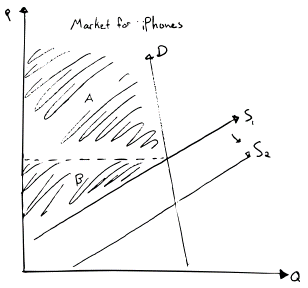
\includegraphics[width=.5\textwidth]{../../figs/iphone3.png}
    \caption{Market for iPhones}
    \label{fig:iphone3}
\end{figure}

\begin{figure}
    \centering
    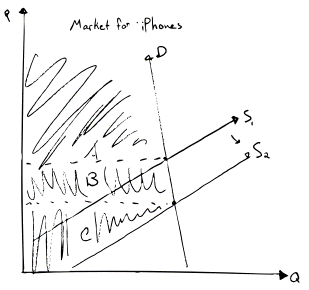
\includegraphics[width=.5\textwidth]{../../figs/iphone4.png}
    \caption{Change to surplus in the market for iPhones}
    \label{fig:iphone4}
\end{figure}

\end{document}